%!TEX root=paper/paper.tex
\section{Problem Definition}\label{sec:det_problem}

\begin{figure}[ht]
\centering
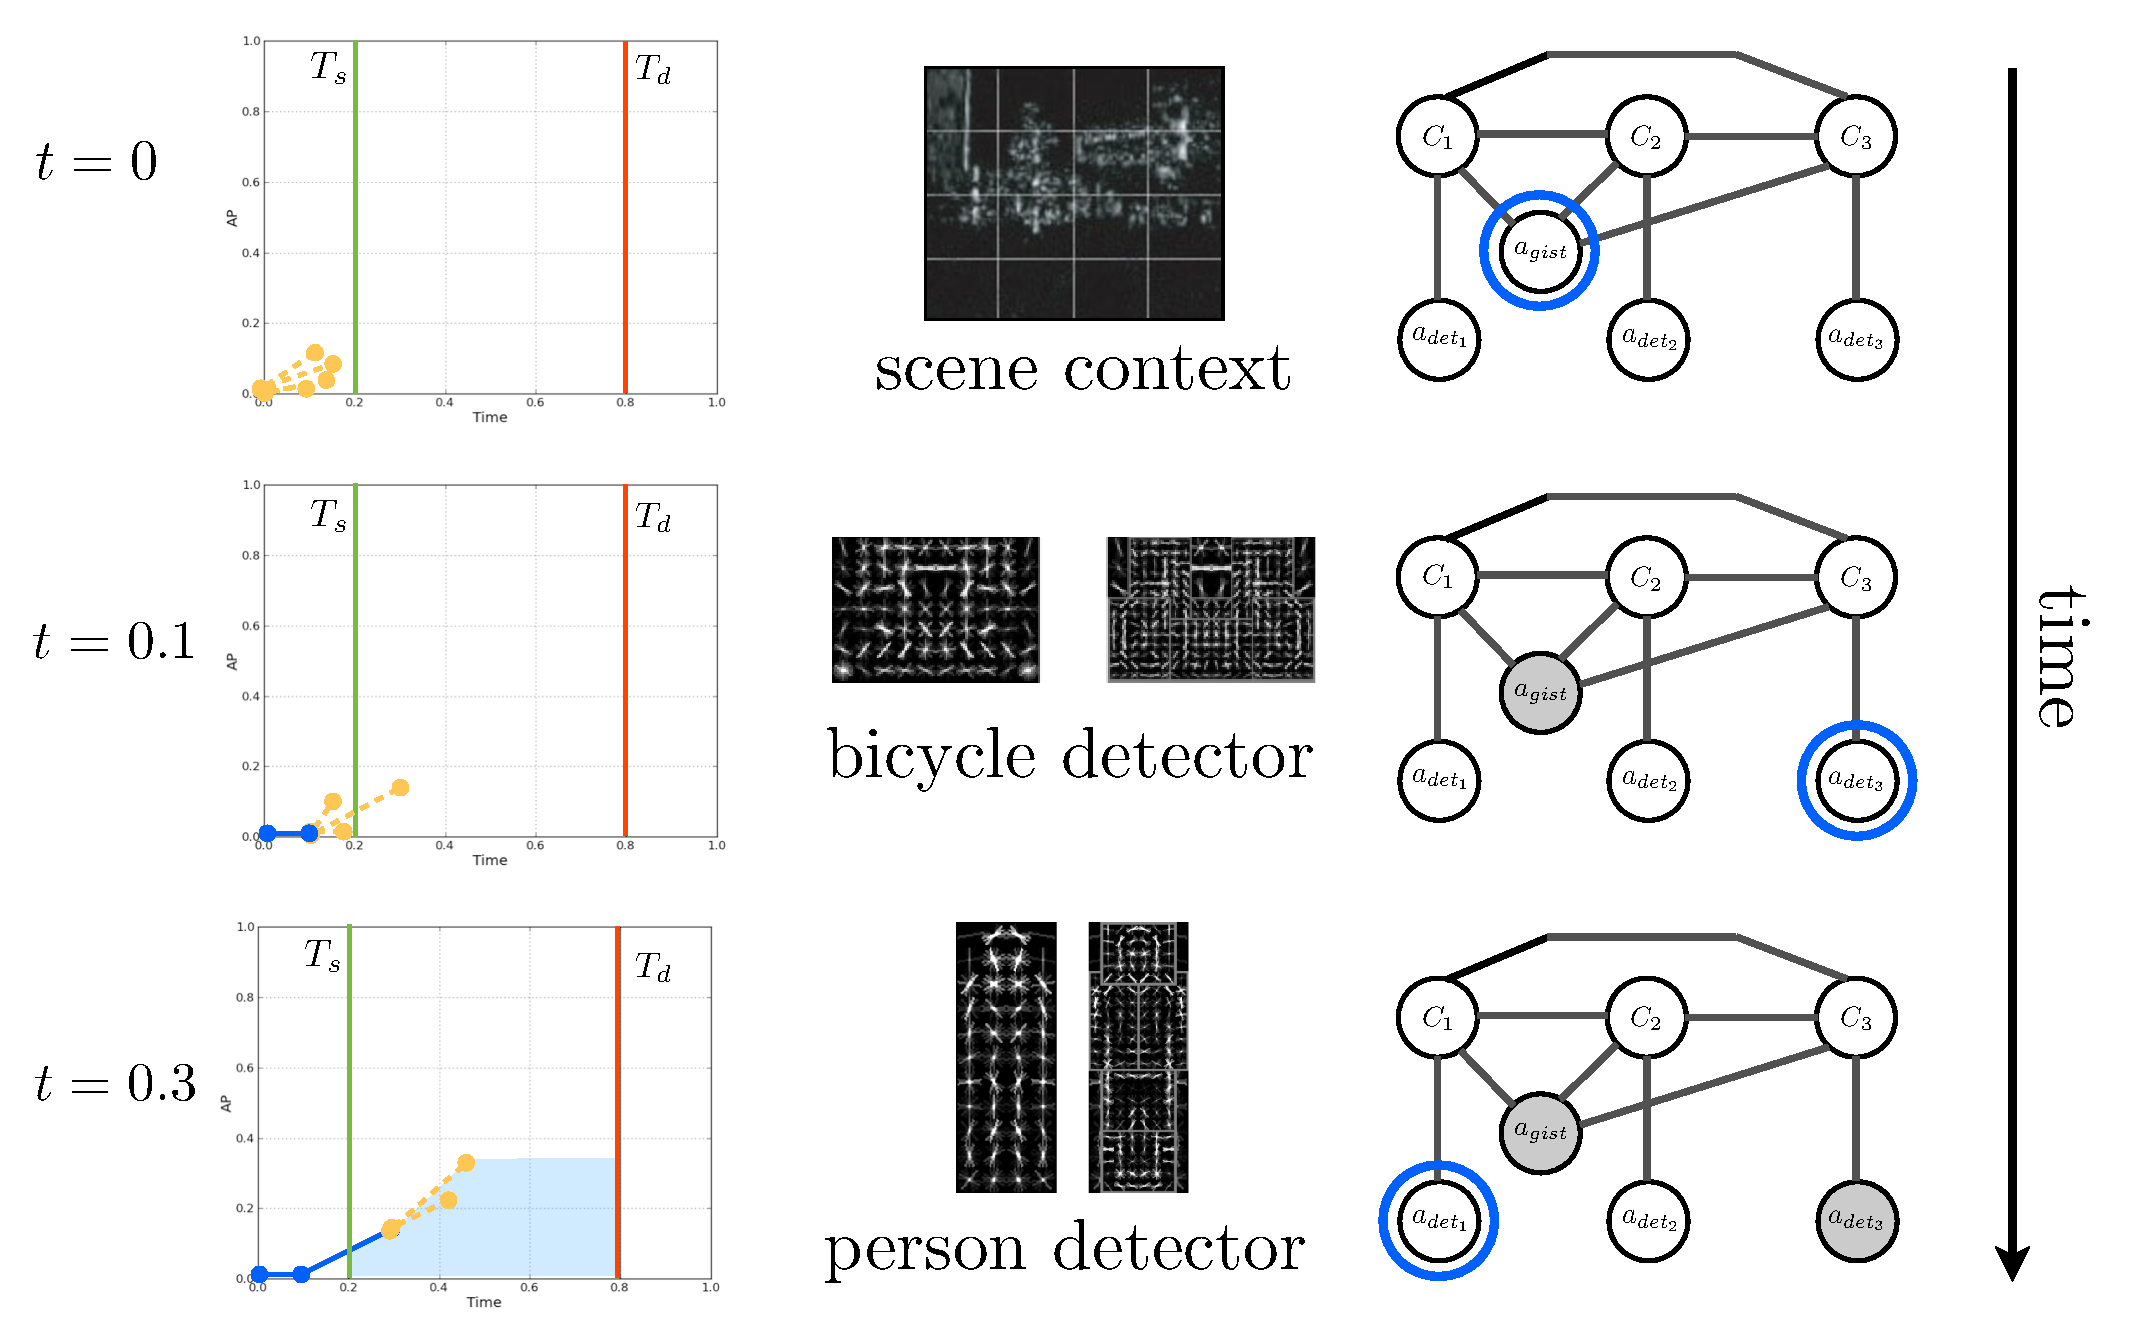
\includegraphics[width=0.86\linewidth]{../../../2011-2012/figures/figure1.pdf}
\caption{
A sample trace of our method.
At each time step beginning at $t=0$, potential actions are considered according to their predicted \emph{value}, and the maximizing action is picked.
The selected action is performed and returns \emph{observations}.
Different actions return different observations: a detector returns a list of detections, while a scene context action simply returns its computed feature.
The \emph{belief model} of our system is updated with the observations, which influences the selection of the next action.
The final evaluation of a detection episode is the area of the \emph{AP vs. Time} curve between given start and end times.
The value of an action is the expected result of final evaluation if the action is taken and the policy continues to be followed, which allows actions without an immediate benefit to be scheduled.
}\label{fig:det_figure1}
\end{figure}


\PM{Types of problems}
We deal with a dataset of images $\mathcal{D}$, where each image $x$ contains zero or more objects.
Each object is labeled with exactly one category label $k \in \{1, \dots, K\}$.
The multi-class, multi-label \textbf{classification} problem asks whether $\mathcal{I}$ contains at least one object of class $k$.
We write the ground truth for an image as $\mathbf{C}=\{C_1, \dots, C_K\}$, where $C_k \in \{0, 1\}$ is set to $1$ if an object of class $k$ is present.
The \textbf{detection} problem is to output a list of bounding boxes (sub-images defined by four coordinates), each with a real-valued confidence that it encloses a single instance of an object of class $k$, for each $k$.
The answer for a single class $k$ is given by an algorithm $\emph{detect}(\mathcal{I},k)$, which outputs a list of sub-image bounding boxes $B$ and their associated confidences.

\PM{Evaluation}
Performance is evaluated by plotting precision vs. recall across dataset $\mathcal{D}$ (by progressively lowering the confidence threshold for a positive detection).
The area under the curve yields the Average Precision (AP) metric, which has become the standard evaluation for recognition performance on challenging datasets in vision \cite{pascal-voc-2010}.
A common measure of a correct detection is the PASCAL overlap: two bounding boxes are considered to match if they have the same class label and the ratio of their intersection to their union is at least $\frac{1}{2}$.
Multi-class performance is evaluated by averaging the individual per-class AP values.
In a specialized system such as the advertising case study from~\autoref{sec:introduction}, the metric generalizes to a weighted average, with the weights set by the \emph{values} of the classes.

\PM{Policy}
Our goal is a multi-class recognition policy $\pi$ that takes an image $x$ and outputs a list of multi-class detection results by running detector and global scene \emph{actions} sequentially.
The policy repeatedly selects an action $a_i \in \mathcal{A}$, executes it, receiving observations $o_i$, and then selects the next action.
The set of actions $\mathcal{A}$ can include both classifiers and detectors: anything that would be useful for inferring the contents of the image.

\PM{Actions}
Each action $a_i$ has an expected cost $c(a_i)$ of execution.
Depending on the setting, the cost can be defined in terms of algorithmic runtime analysis, an idealized property such as number of \emph{flops}, or simply the empirical runtime on specific hardware.
We take the empirical approach: every executed action advances $t$, the \emph{time into episode}, by its runtime.
The specific actions we consider in the following exposition are detector actions $a_{{det}_i}$, where ${det}_i$ is a detector class $C_i$, and a scene-level context action $a_{gist}$, which updates the probabilities of all classes.
Although we do not showcase this here, note that our system easily handles multiple detector actions per class.

\PM{Anytime metric}
As shown in \autoref{fig:det_figure1}, the system is given two times: the setup time $T_s$ and deadline $T_d$.
We want to obtain the best possible answer if stopped at any given time between the setup time and the deadline.
A single-number metric that corresponds to this objective is the area captured under the curve between the start and deadline bounds, normalized by the total area.
We evaluate policies by this more robust metric and not simply by the final performance at deadline time for the same reason that Average Precision is used instead of a fixed Precision vs. Recall point in the conventional evaluations.
Additionally, maximizing this single-number metric corresponds to maximizing Anytime performance.
